\documentclass[lettersize,journal]{IEEEtran}
\usepackage{amsmath,amsfonts}
\usepackage{array}
\usepackage{textcomp}
\usepackage{url}
\usepackage{verbatim}
\usepackage{graphicx}
\usepackage[catalan]{babel}
\usepackage{lipsum}

\renewcommand{\figurename}{\textbf{Figura}}

\renewcommand{\abstractname}{Resum}
\renewcommand{\IEEEkeywordsname}{Paraules clau}

\begin{document}

\title{Disseny d'una Eina per al Tractament i \\ Visualització de les Dades d'Accés a un Repositori}
\author{\textbf{Omar Briqa} \\ \vspace{5pt} Escola Politècnica Superior d'Enginyeria de Vilanova i la Geltrú}
\maketitle

\begin{abstract}
\end{abstract}

\begin{IEEEkeywords}
    DSpace, Metadades, UPCommons, Grafana, InfluxDB, MongoDB, Registre d’accés.
\end{IEEEkeywords}


\section{Introducció}\label{sec:introduction}
\IEEEPARstart{I} ntroducció

\section{Processament de les dades}\label{sec:data-processing}
La primera etapa del nostre projecte consisteix a processar les dades.
Volem respondre a preguntes com: què són aquestes dades, com estan estructurades, quina informació proporcionen, com les podríem tractar\dots
Durant aquest procés, analitzarem tots els registres d'accés, emmagatzemats al nostre servidor de treball.
Concretament, parlem dels registres d'accés des del primer dia de l'any 2006 fins al darrer accés de l'any 2023.

A causa de la gran quantitat de dades, hem de dissenyar un procés que analitzi tots aquests registres de manera automatitzada.
Aquest procés ha de tractar diverses casuístiques dels registres, ja que els servidors no només registren accessos a la plataforma d'UPCommons, sinó que moltes més coses.
Accessos a recursos web, repeticions de registres, alguns amb el seu format alterat, són alguns casos que hem anat trobant pel camí.
Un cop aclarits tots els casos, proposem un disseny modular, independent de la seva implementació, per dur a terme aquesta anàlisi.

L'objectiu d'aquest és convertir els \textit{logs} del format específic amb el qual s'enregistren a la plataforma d'UPCommons, a un altre més operable, on també hi hem afegit informació significativa que ens serà útil per als passos posteriors.
Saber si el \textit{log} és una cerca a la plataforma, un accés a un recurs o d'altre tipus, i marcar-ho al mateix registre pot simplificar molt el seu tractament.

Per altra banda, processarem també les metadades.
Aquestes són les etiquetes presents a cadascun dels recursos d'UPCommons, amb l'objectiu d'enriquir la informació d'aquests.
Els autors, la descripció del recurs, la data de pujada, el departament responsable, el tipus de document o més, es troben inclosos.
La plataforma d'UPCommons està basada en el programari de codi obert DSpace, plataforma per la construcció i gestió de repositori digitals, una de les més utilitzades [REF].
El format de les metadades és el DIM (DSpace Intermediate Metadata), que es basa en l'agregació d'un qualificador al format Dublin Core ja existent.
Per exemple, l'autor principal d'un recurs ve definit per la metadada:
\begin{center}
    {dc.contributor.author}
\end{center}

Les metadades les podrem trobar a un servidor de desenvolupament on només hi són emmagatzemadaes aquestes.
Utilitzarem el protocol OAI-PMH (Open Archives Initiative Protocol for Metadata Harvesting) per descarregar aquestes.
Una característica interessant d'aquest servidor, i que no tots els servidors OAI tenen, és la funcionalitat del control de flux mitjançant \textit{resumptionToken}.

Els verbs del protocol OAI-PMH per obtenir les metadades no poden obtenir totes les metadades d'una tirada, ja que no és gens pràctic a causa del seu gran nombre.
Com a conseqüència, retornen un valor que indica en quin punt de la descàrrega ets, permetent la modularització de l'obtenció de les metadades.

Implementarem aquest procés amb la llibreria Sickle [REF], encara que gràcies a la simplicitat d'aquest protocol podríem dur a terme sense la necessitat de llibreries externes.
Com a primera fase, les estructurarem localment en el nostre sistema de fitxers.
Més endavant les migrarem a un sistema gestor de bases de dades.


\section{Emmagatzemament de les dades}\label{sec:data-storing}
\subsection{Sistemes gestors de bases de dades}\label{subsec:data-storing-requirements}
Un cop tenim la informació processada, necessitem una solució d'emmagatzemament de dades per poder consultar aquestes dades d'una forma simple, eficient i consistent.
La resposta sembla ser senzilla: utilitzar bases de dades.
Tot i així, hem de respondre a les següents preguntes: que emmagatzemem exactament, quin format utilitzem, quina o quines bases de dades utilitzarem i quines són les característiques i funcionalitats necessàries.

Per cada secció del projecte (\textit{logs} i metadades) s'han considerat diverses opcions, valorant els seus punts a favor i en contra.
De forma general, per la base de dades que emmagatzemi els registres d'accés, les característiques ideals són:
\begin{itemize}
    \item Base de dades de codi obert.
    \item Enfocada a tractar registres d'accés, o elements que ocorren en un cert punt de temps (bases de dades de sèries temporals).
    \item Estigui ben documentada, actualitzada i mantinguda per una comunitat activa d'usuaris, desenvolupadors\dots
    \item Capacitat de processar grans quantitats de dades.
    \item Capacitat d'allotjar la base de dades localment al nostre servidor de treball.
\end{itemize}

La solució final fou triar InfluxDB.
Aquesta opció a més de complir amb totes les característiques anteriors, incorpora una funcionalitat d'indexació per paràmetres interessant.
Podrem indexar els paràmetres freqüents que vam afegir als registres en l'etapa de processament per després optimitzar la cerca.
Podrien ser la tipologia de \textit{log} (cerca, accés a recurs\dots), els paràmetres de la petició d'HTTP dels \textit{logs}, el codi de resposta de la petició\dots
Tot depèn del processament que s'hagi fet anteriorment, i la semàntica que se li hagi associat a un \textit{log}.

En relació amb la base de dades per emmagatzemar les metadades, com la quantitat d'aquestes és de quatre ordres de magnitud inferior que la dels \textit{logs}, els requisits no són tan estrictes.
En canvi, el requisit més important és la flexibilitat del model de dades.
Les metadades poden tenir valors múltiples, fet que faria incompatible l'ús d'algunes bases de dades relacionals.

Pel fet que durant l'obtenció de les metadades del servidor OAI, aquestes estiguin en format XML (Extensible Markup Language), podríem convertir-les a un format d'un document de parelles clau-valor.
El sistema gestor de bases de dades més popular basat en documents és MongoDB.
Senzill d'utilitzar i de configurar, aquesta va ser la nostra decisió per emmagatzemar les metadades.

\subsection{Procés d'abocament de les dades}\label{subsec:data-storing-process}

El procés d'abocament de les metadades s'ha fet continuadament del de processament de dades.
L'automatització dels dos processos ens ha permès treballar concurrentment en altres bandes del projecte, mentre monitoràvem puntualment l'estat d'aquest.
S'ha fet un abocament per cada base de dades.
Encara que l'objectiu no era optimitzar al màxim i reduir aquest temps, a causa del gran nombre de \textit{logs} hem dut a terme una sèrie de millores recomanades pel mateix InfluxDB [REF].

El resultat de l'abocament dels \textit{logs} conclou amb els resultats de la taula~\ref{tab:table1}.

\begin{table}[!t]
    \caption{Resultat de l'abocament dels logs}\label{tab:table1}
    \centering
    \begin{tabular}{|l|r|}
        \hline
        \textbf{2006-2023} & Total\\
        \hline
        Nº total de \textit{logs}       & 1.922.392.760\\
        \hline
        Accés a recursos UPCommons      & 1.208.133.268\\
        \hline
        Cerques a UPCommons             & 179.937.769\\
        \hline
        Accés a recursos web descartats & 430.789.238\\
        \hline
        Altres tipus de \textit{logs}   & 107.198.724\\
        \hline
        Errors de processament          & 552\\
        \hline
        Duració (minuts)                & 1.977,13\\
        \hline
    \end{tabular}
\end{table}

Algunes consideracions:

\begin{itemize}
    \item El nombre d'errors de processament irreversibles és sorprenentment baix.
    Això és degut al fet que la plataforma registra els \textit{logs} de forma correcta, i que l'eina que hem dissenyat els processa correctament.
    \item L'abocament total ha trigat un total de 1977 minuts, que correspon a aproximadament 33 hores.
    De mitjana, cada \textit{log} tarda 61 \(\mu s\).
\end{itemize}

El resultat de l'abocament de les metadades al base de dades MongoDB conclou amb els resultats de la taula~\ref{tab:table2}.
El volum total d'aquestes dades (648 MB) va fer possible realitzar aquest abocament prèviament al sistema de fitxers del servidor de treball.
D’aquesta manera evitem tornar a fer les peticions al servidor en cas que el bolcat falli, o les dades pateixin algun tipus d’alteració o corrupció.
El resultat d'aquest abocament es mostra a la taula~\ref{tab:table3}

\begin{table}[!t]
    \caption{Resultat de l'abocament de les metadades\label{tab:table2}}
    \centering
    \begin{tabular}{|c|c|c|}
        \hline
        MongoDB & Nº total de metadades & Duració (segons)\\
        \hline
        \textbf{Total} & 242.555 & 38,2050559520721\\
        \hline
    \end{tabular}
\end{table}

\begin{table}[!t]
    \caption{Resultat de l'abocament de les metadades\label{tab:table3}}
    \centering
    \begin{tabular}{|c|c|c|}
        \hline
        Servidor de treball & Nº total de metadades & Duració (minuts)\\
        \hline
        \textbf{Total} & 242.555 & 20,95360236565\\
        \hline
    \end{tabular}
\end{table}

\section{Servidor de treball}\label{sec:server-ostia}
\lipsum[1]

\section{Anàlisi i visualització de les dades}\label{sec:data-visualization}
Un cop finalitzats tant l’anàlisi com l’emmagatzemament de les dades, arribem a la part de l’anàlisi i la visualització de les dades.
Per mostrar el potencial d’aquesta eina, hem definit uns quants casos d’ús prou representatius que poden servir com a exemple.

Utilitzem el programari d'observabilitat Grafana com a eina de suport.
Amb aquesta eina generarem informes visuals dels diversos casos d'ús que vulguem tractar.
Per cada cas d'ús, els nostres exemples es basen en definir del què tracta, que analitzarem, com ho representarem i la discussió dels resultats.

N'hem definit tres:
\begin{itemize}
    \item Recurs més accedit durant un període de temps.
    \item Accessos amb el seu contingut alterat.
    \item Condicions d’accés dels accessos a recursos de l’EPSEVG.
\end{itemize}

A continuació detallarem el tercer cas d'ús, que tracta sobre les condicions d'accés dels accessos a recursos de l'EPSEVG, mostrant la funcionalitat completa de l'eina.

\textit{\textbf{Precondicions}}

Hem de tenir els \textit{logs} emmagatzemats a la base de dades InfluxDB.
Això ja s'ha fet a l'emmagatzemament de les dades.

També hem de tenir marcats els \textit{logs} que siguin un accés a un recurs d'UPCommons, d'aquesta manera podem descartar tots els altres registres durant aquesta anàlisi.
Ho hem fet al processament de les dades.

\textit{\textbf{Definició}}

Donat el període de temps del primer de desembre del 2023, volem saber quines són les condicions d'accés dels accessos als recursos de l'EPSEVG.

Volem determinar si són d'accés obert, restringits per decisió de l'usuari, restringits a la comunitat académica\dots

\textit{\textbf{Anàlisi simplificat}}

Obtenim tots els accessos a recursos d'aquest dia de la nostra base de dades de \textit{logs}, filtre només aquells que siguin accessos a recursos.

A continuació busquem a la base de dades de les metadades amb l'identificador del recurs, si aquest està relacionat amb l'EPSEVG.
Aquest filtre ho fem amb la metadata:
\begin{center}
    {dc.audience.mediator}
\end{center}

Si ho està, obtenim el tipus d'accéss d'aquest recurs, amb la metadata corresponent, i ho emmagatzemem.
Aquesta informació es troba al valor de la metadata:
\begin{center}
    {dc.rights.access}
\end{center}

\textit{\textbf{Resultat}}

Amb la informació prèviament processada, utilitzarem Grafana per representar visualment la tipologia d'accessos.

Les diferents condicions d'accés d'aquest període per accessos a recursos, representades a la figura~\ref{fig:log-access-type}, són:
\begin{itemize}
    \item Verd: recurs d'accés obert.
    \item Groc: recurs restringit per decisió de l'autor.
    \item Blau: recurs restringit per acord de confidencialitat.
    \item Vermell: recurs restringit a la comunitat acadèmica de la UPC.
    \item Taronja: recurs restringit a la comunitat acadèmica del CSUC (Consorci de Serveis Universitaris de Catalunya).
\end{itemize}

Les condicions d'accés més habituals són aquelles on més usuaris poden accedir.

Aquestes són l'accés obert i l'accés restringit a la comunitat acadèmica de la UPC.

Cal remarcar que tots els exàmens són restringits a la comunitat acadèmica de la UPC.
\begin{itemize}
    \item Aquell dia es van registrar un total de 2001 accessos a recursos restringits a la comunitat acadèmica de la UPC, dels quals 1961 eren accessos a exàmens.
\end{itemize}

Els menys accedits són aquells d'accés restringit a un públic petit.

\begin{figure}[!t]
    \centerline{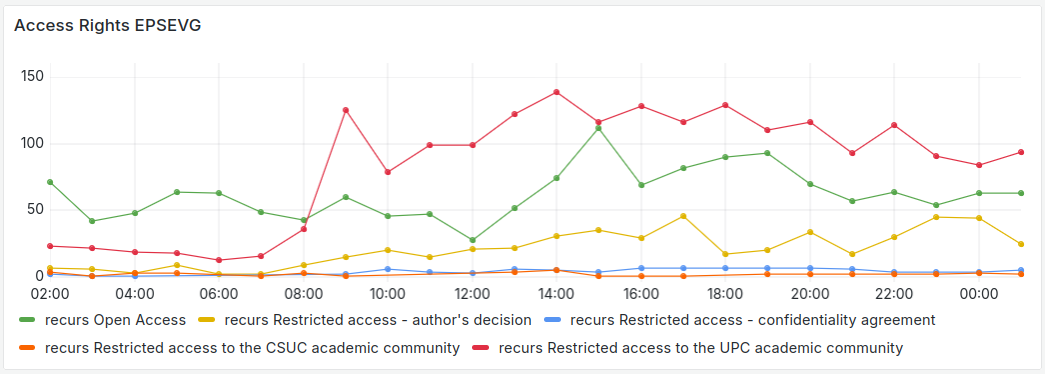
\includegraphics[width=0.5\textwidth]{figures/access-rights-epsevg}}
    \caption{Condicions d'accés dels accessos a recursos de l'EPSEVG el primer de desembre del 2023.}\label{fig:log-access-type}
\end{figure}

\section{Conclusions}\label{sec:conclusions}

\begin{thebibliography}{1}
\bibliographystyle{IEEEtran}

\bibitem{ref1}
    {\textit{Mathematics Into Type}}. American Mathematical Society. [Online]. Available: https://www.ams.org/arc/styleguide/mit-2.pdf
\end{thebibliography}

\end{document}
